\documentclass[draft, ../thesis.tex]{subfiles}

\begin{document}
    \chapter{Introduction}
    
    In this thesis, we propose a novel methodology for solving the hierarchical classification problem for multi-class classification problems in supervised machine learning. This chapter will motivate and introduce our research question, introduce the key concepts underlying our approach, and outline the structure of the thesis.
    
    \section{Motivation}
    \label{motivation}
    Suppose that we had a data set containing images of cats, golden retrievers, and Labrador retrievers and our goal is to perform image classification. For reference an example of each of these species is shown in Figure \ref{fig:animal_compare}. 
    
    \begin{figure}
    	\centering
    	\begin{subfigure}[b]{.30\linewidth}
    		\centering
    		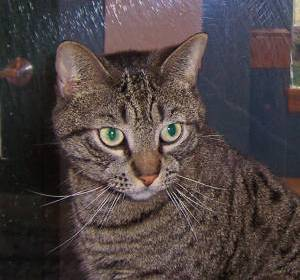
\includegraphics[width=.7\linewidth]{images/cat}
    		\caption{Cat}
    	\end{subfigure}
    	\begin{subfigure}[b]{.3\linewidth}
    		\centering
    		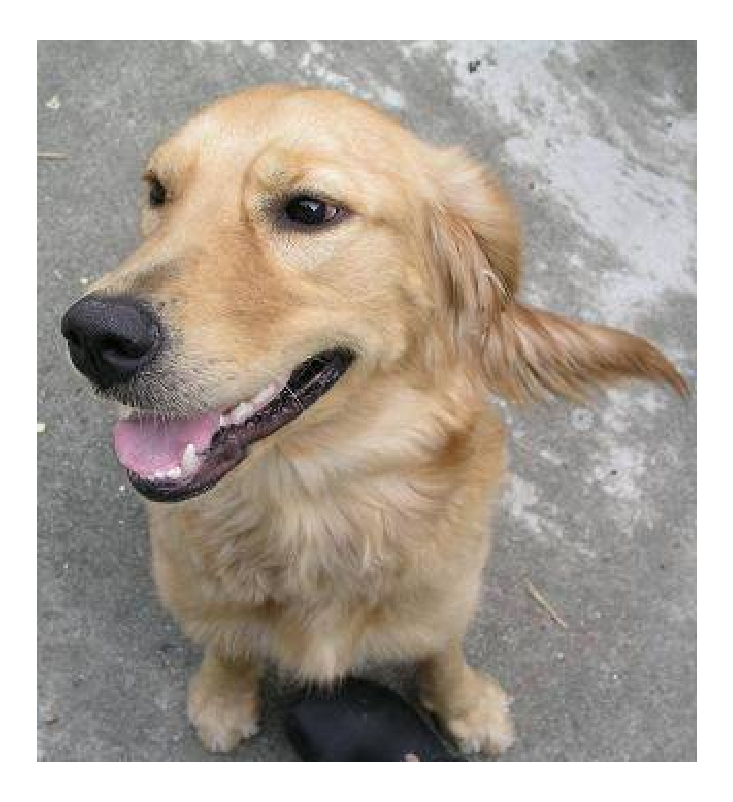
\includegraphics[width=.7\linewidth]{images/golden}
    		\caption{Golden Retriever}
    		\label{fig:golden}
    	\end{subfigure}
    	\begin{subfigure}[b]{.3\linewidth}
    		\centering
    		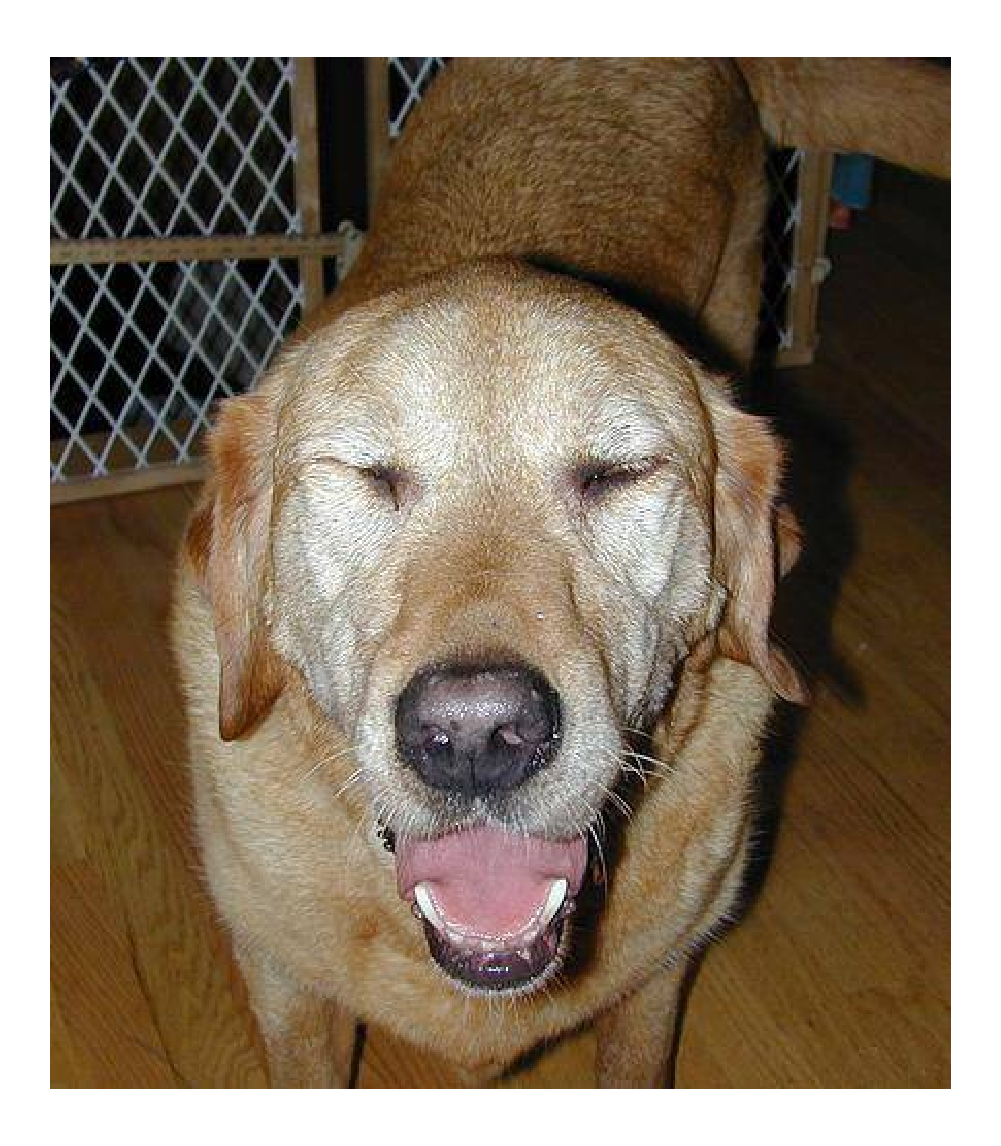
\includegraphics[width=.7\linewidth]{images/lab}
    		\caption{Labrador Retriever}
    		\label{fig:lab}
    	\end{subfigure}
    	\caption{Visual Comparison of a Cat, Golden, and Labrador retriever}
    	\label{fig:animal_compare}
    \end{figure}
    
    Intuitively, we expect a classifier would be able to distinguish an image of cat versus the other two dog breeds. Cats do not look like golden or Labrador retrievers. However, it is quite likely that our model would confuse the dog breeds; Figures \ref{fig:golden} and \ref{fig:lab} look quite similar to one another. While there are differences between them (one example being that golden retrievers typically have wavier fur) this is a subtle visual cue that would probably only be distinguished if we had a model that specialized in telling the differences between goldens and labs.
    
    Turning to another example, suppose that I had a dataset consisting of satellite images from buildings and locations of interest. Moreover, suppose that we wanted to classify the picture shown in Figure \ref{fig:prison01rgb} as its label, a prison.
    
    \begin{figure}
    	\centering
    	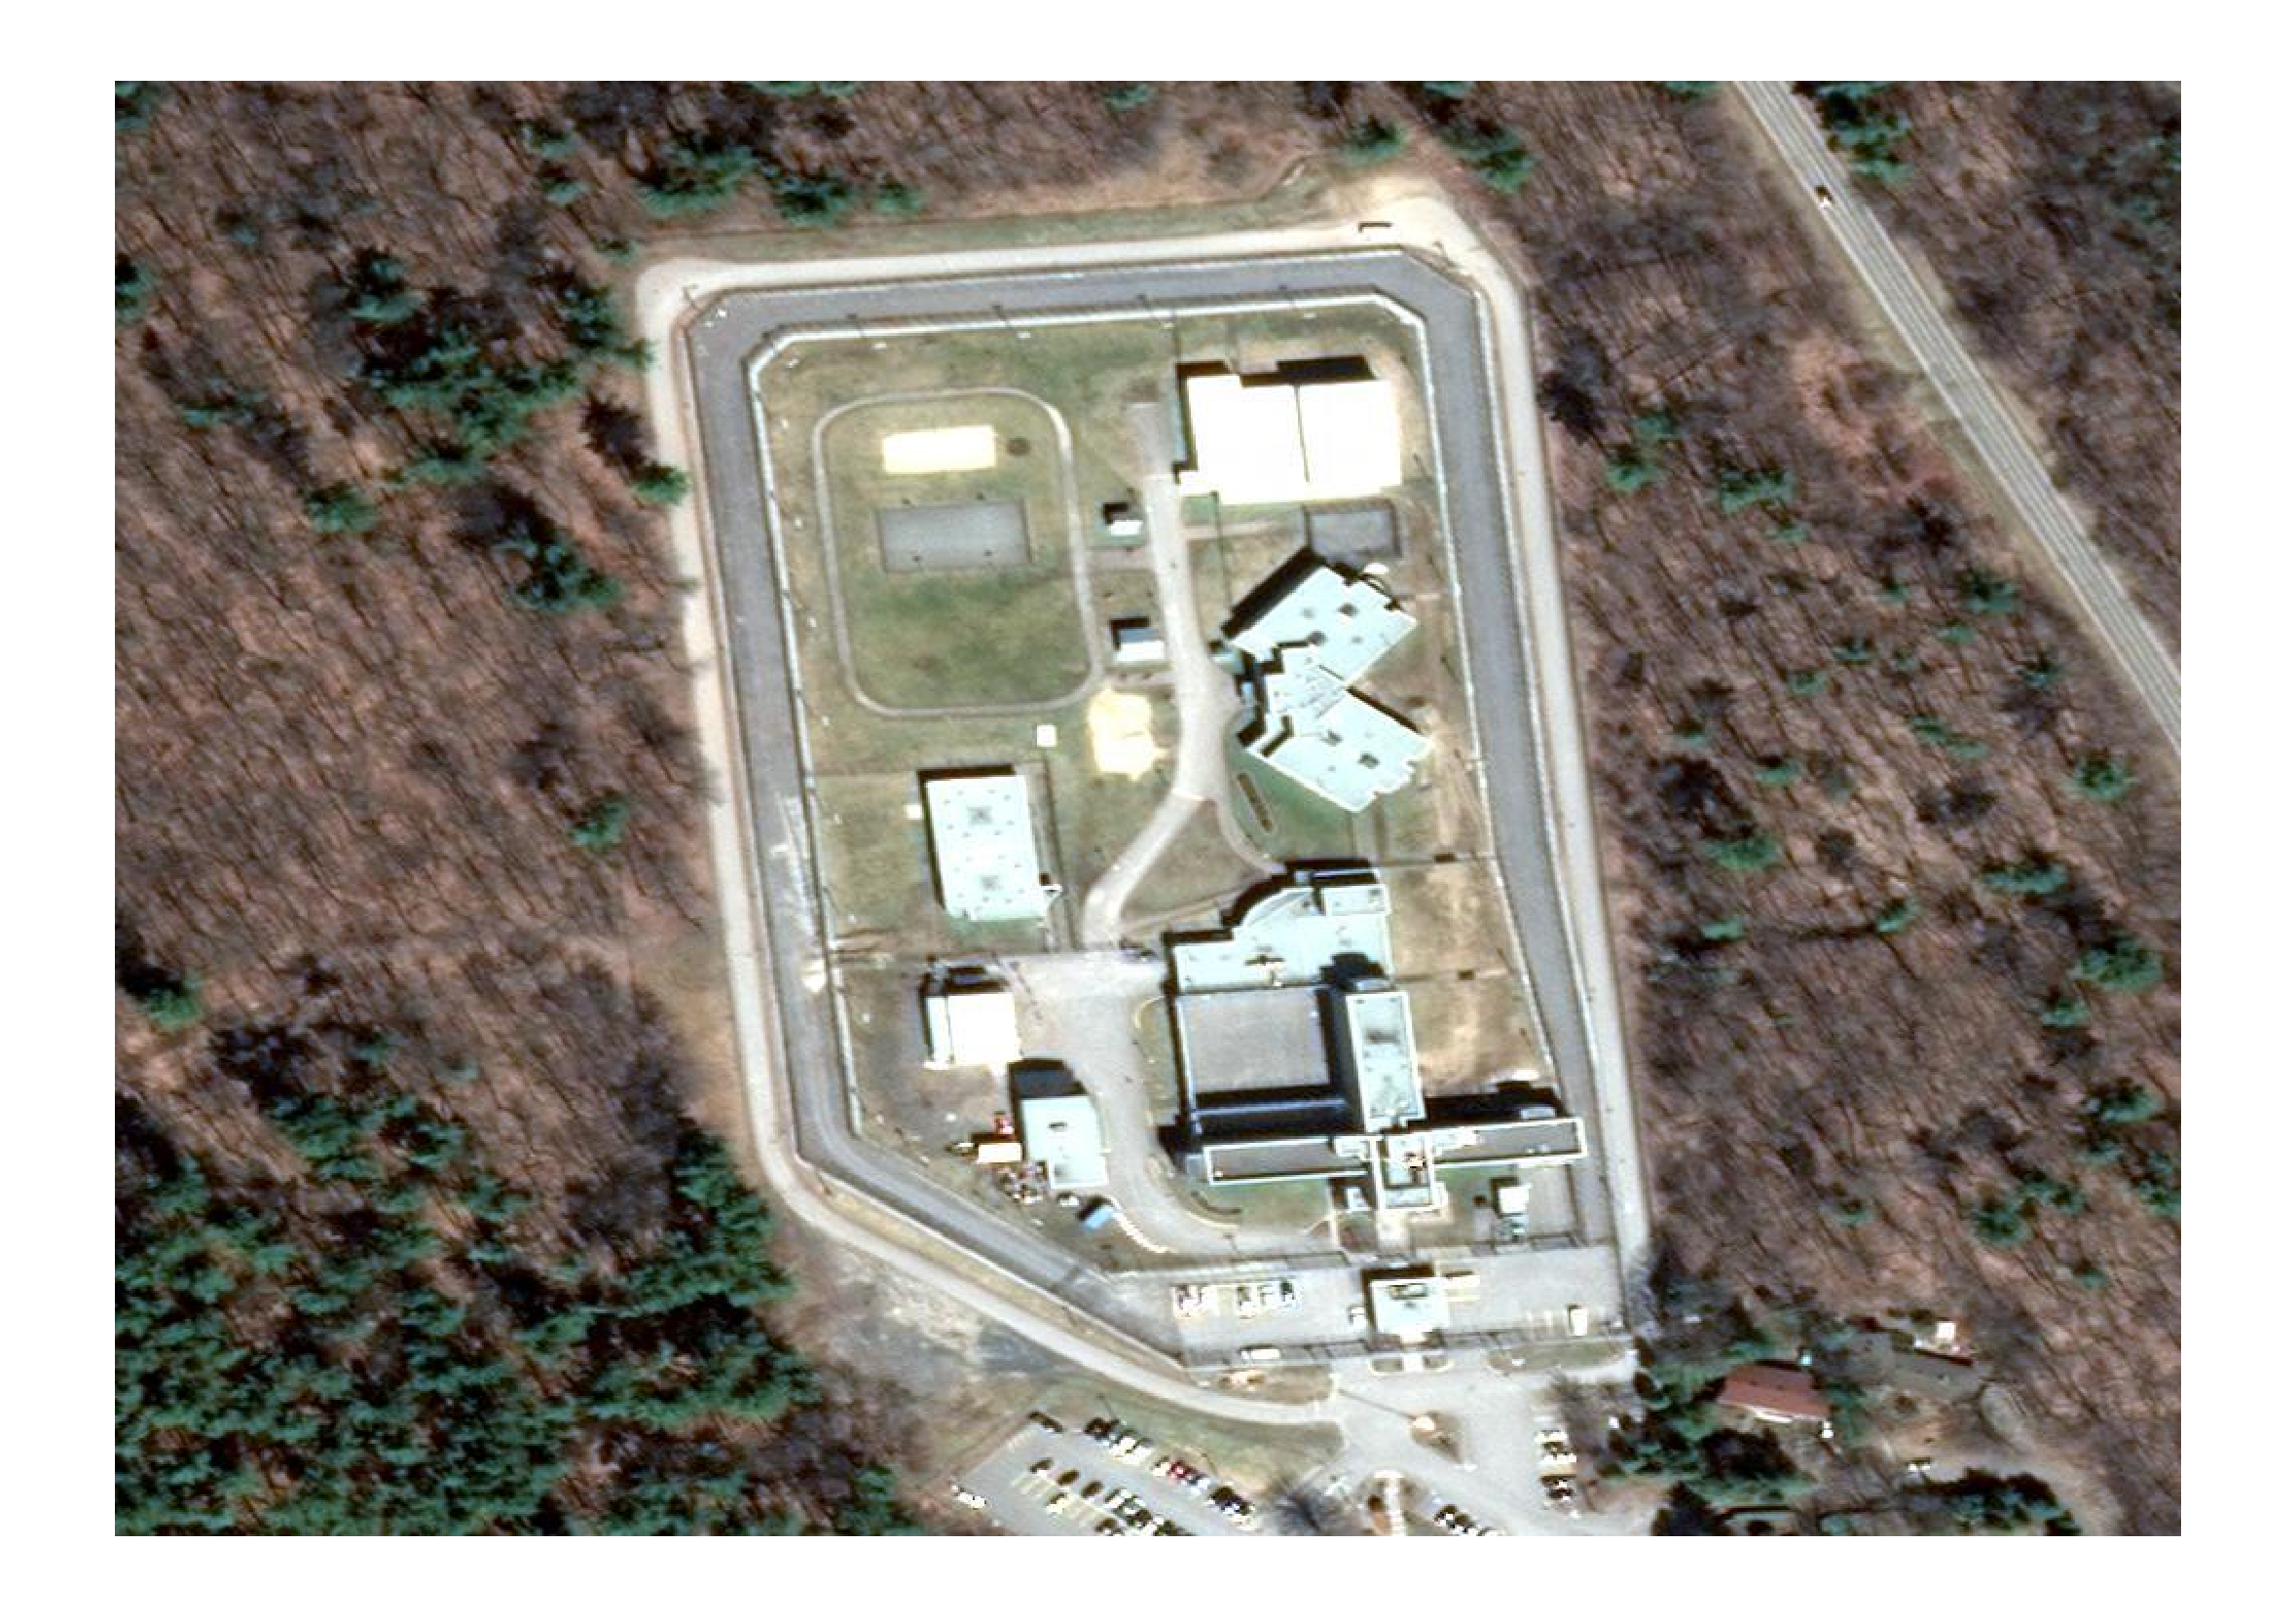
\includegraphics[width=0.7\linewidth]{images/prison}
    	\caption{Example Prison Satellite Image}
    	\label{fig:prison01rgb}
    \end{figure}
    
    The dataset where Figure \ref{fig:prison01rgb} was drawn from has $62$ label choices and those are listed in Appendix \ref{fmow_labels}. Similar to the pet example, certain labels are not likely to be confused with the prison such as airports, barns, and nuclear power plants. However, asking our model to discriminate between, say the prison and a military facility might be more difficult. Again the two classes share a number of visual similarities from space; both have a gate around the main area, both have plain architecture, etc. Nevertheless, if our model only had to discriminate between those two classes, the classification task would be much easier. We could use features specific to those two classes, that could not be used in the traditional multi-class setting because it would lead to over-fitting. 
    
    Looking at the two examples we have provided a couple themes jump out. First, when dealing with multi-class classification problems, oftentimes a given class is confused with a small subset of other labels. Second, it is typically easier to break classification problems up into small groups which allow us to learn more specialized functions versus attempting to predict everything at once. Those ideas motivate a technique known as ``hierarchical classification.'' An example of a hierarchical classifier (HC) is shown in Figure \ref{fig:hierarchicalclassifier}.
    
    \begin{figure}
    	\centering
    	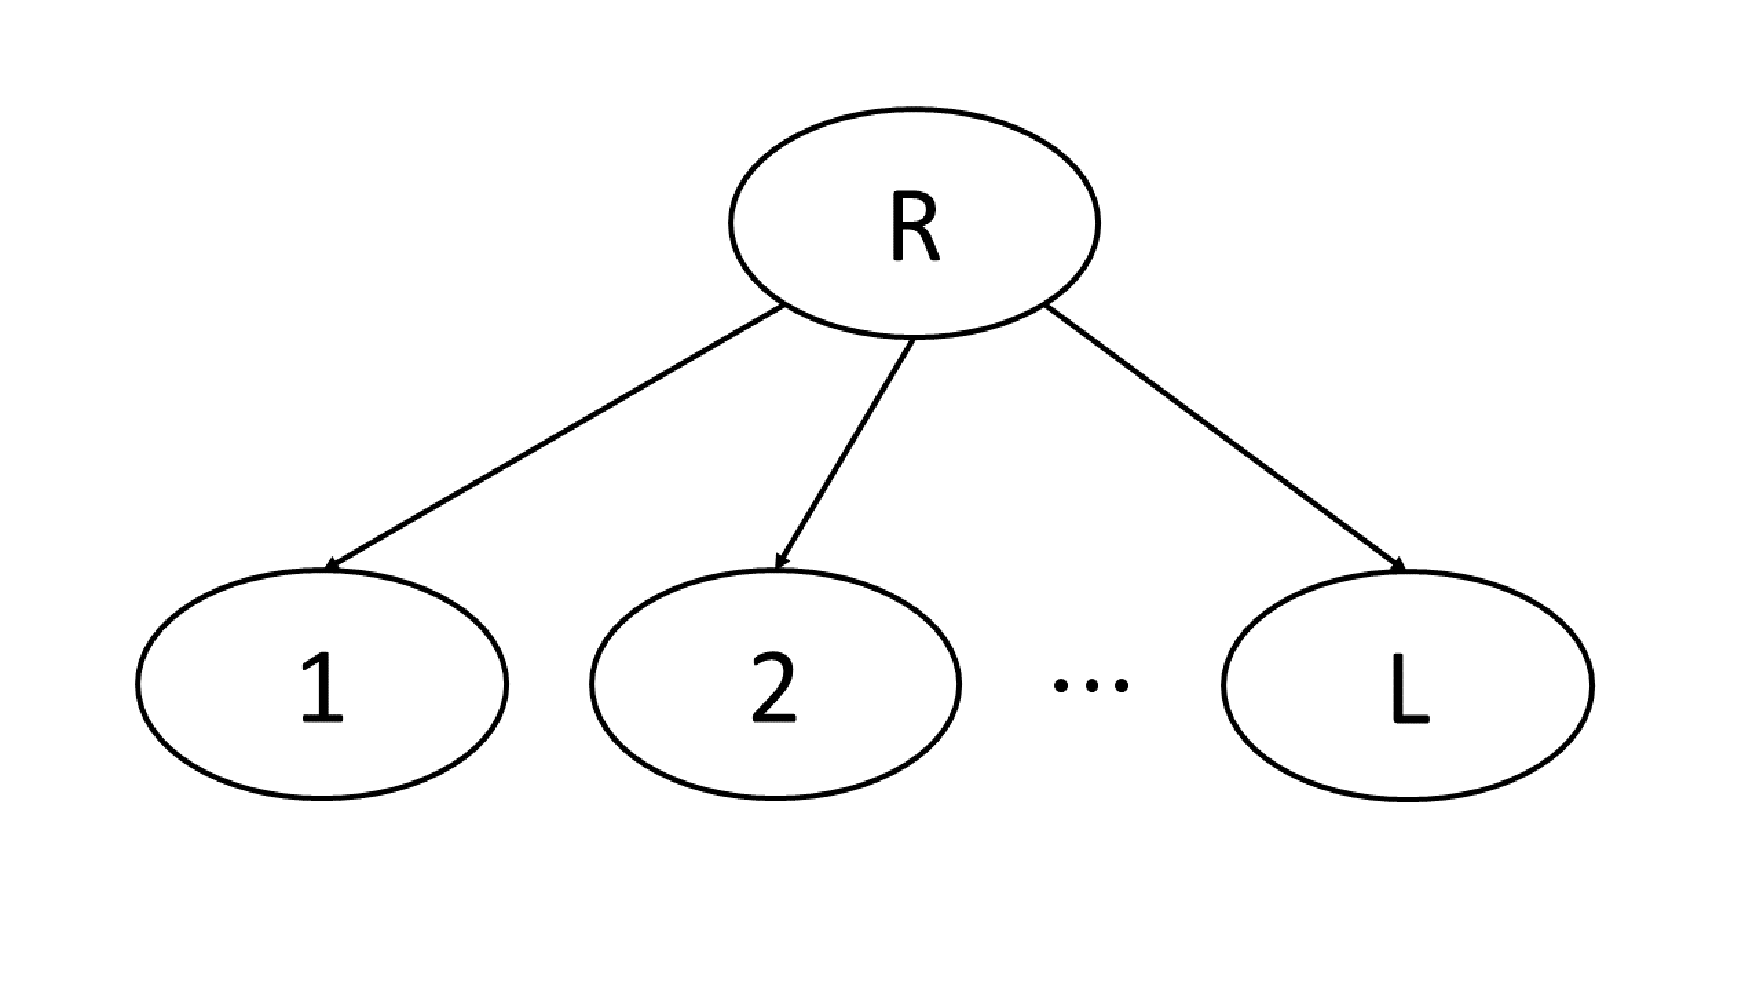
\includegraphics[width=0.7\linewidth]{images/hierarchical_classifier}
    	\caption{Standard Hierarchical Classifier Graph}
    	\label{fig:hierarchicalclassifier}
    \end{figure}
    
    At a high level, an HC uses either an inferred or provided label hierarchy to first predict whether a label belongs to a given ``meta-class.'' (a subset of the classes that have been grouped together). Then for each of the meta-classes, represented as the leaves in Figure \ref{fig:hierarchicalclassifier}, one can train a classifier to specialize for those particular labels. The main idea behind hierarchical classification is that by learning specialized functions for a small subset of labels, it is possible to improve overall classifier performance, but at the cost of increased training time. 
    
    As we stated previously, to train an HC, one needs to have a label hierarchy to build the classifier tree. For the example involving cats and dogs, while there is not an explicit label map provided, one clear partition is to group the two dog breeds together as one meta-class and have the images of cats by themselves. Conversely for the satellite imagery example though, the grouping is not obvious. For some of the labels, such as all of the airport classes, it would be sensible to group them with one another. Nevertheless, for even a relatively small scale problem of $62$ labels, if one asked experts from various fields, it is quite likely that we would get a variety of answers regarding how the labels should be organized with one another. Now imagine that one had a data containing $1000$ labels. In many cases, it would be both impractical and infeasible for an expert to encode the label relation, by hand, for a problem of that size. The point being is that if one does not know the label hierarchy a-priori (as is often assumed in the hierarchical classification literature) and we are dealing with a problem of even modest size, one's ability to encode a sensible label hierarchy diminishes drastically.  
    
    Along with the problem of an unknown label hierarchy, we have the issue of training the HC. While earlier we discussed and in Figure \ref{fig:hierarchicalclassifier} we describe the standard approach of making sequential classifications according to a proscribed graph as defined by the label hierarchy, it is not clear that this the best way to approach this problem. By construction, any error made the root node, denoted as ``R'' in Figure \ref{fig:hierarchicalclassifier}, cannot be recovered in the leaves. Moreover, by training each component independently of one another, the leaves and root cannot provide feedback to improve the overall tree loss; they are simply minimizing the loss for that particular node. 
    
    These two main issues: how to find a label partition when it is not known a-priori and how to design a HC form the central focus of this thesis. 
    
    \section{Problem Statement}
    \label{problem_statement}
    The central problems of this thesis are
    
    \begin{enumerate}
    	\item How do we group similar labels together?
    	\item How do we train a HC using a fixed label hierarchy?
    \end{enumerate}
    
    For the first question, we are interested in designing an algorithm which is able to take in data of the form $\mathcal{D} = \{(\mathbf{x}_i, y_i)\}_{i=1}^n$ where $\mathbf{x} \in \R^p$ and $y \in \{1, 2, \ldots, C\}$ and find a label map $f: \{1, 2, \ldots, C\} \longrightarrow \{1, 2, \ldots, L\}$ where $L$ is given as an input to the function. 
    
    For the second question, assuming we have the label partition, $\mathbf{Z}$, how we can use $\mathbf{Z}$ to help find a function $g: \mathbf{x} \longrightarrow y$ which avoids the pitfalls discussed in Section \ref{motivation}.
    
    To test these questions we primarily use image classification datasets. We selected image data because in many commonly used benchmarks, we observe there exist subsets of the labels which exhibit some degree of similarity to one another thereby making discriminating these classes more difficult.
    
    \section{Thesis Organization}
    Using the two main questions outlined in Section \ref{problem_statement} we will describe how the remainder of the thesis is organized.
    
    \begin{itemize}
    	\item In Chapter 2 (Background), we contextualize our work by providing previous approaches to the hierarchical classification problem and common machine learning (ML) techniques used to solve image classification tasks. 
    	
    	\item In Chapter 3 (Methods), we define our approach to solving the question of first how to group similar labels together and then using the label partition how we can then train a HC.  
    	
    	\item In Chapter 4 (Experiments and Analysis), we test our methods against the existing state of the art on a number of benchmark and novel datasets. 
    	
    	\item In Chapter 5 (Conclusions), we conclude and propose future avenues for research.
    \end{itemize}
\end{document}

